\documentclass{article}
\usepackage{microtype}
\usepackage{graphicx}
\usepackage{subfigure}
\usepackage{booktabs}
\usepackage{hyperref}
\usepackage{amsmath}
\usepackage{amssymb}
\usepackage{mathtools}
\usepackage{amsthm}
\usepackage[capitalize,noabbrev]{cleveref}
\usepackage[accepted]{icml2025}
\usepackage{algorithm}
\usepackage{algorithmic}
\theoremstyle{plain}
\newtheorem{theorem}{Theorem}[section]
\newtheorem{proposition}[theorem]{Proposition}
\newtheorem{lemma}[theorem]{Lemma}
\newtheorem{corollary}[theorem]{Corollary}
\theoremstyle{definition}
\newtheorem{definition}[theorem]{Definition}
\newtheorem{assumption}[theorem]{Assumption}
\theoremstyle{remark}
\newtheorem{remark}[theorem]{Remark}

\icmltitlerunning{Advancing Knotted Protein Design with ESM3}

\begin{document}

\twocolumn[
\icmltitle{Advancing Knotted Protein Design with ESM3:\\ Guided Generation and Topological Insights}

\begin{icmlauthorlist}
\icmlauthor{Petr Simecek}{inst1}
\icmlauthor{Eva Marsalkova}{inst1,inst2}
\end{icmlauthorlist}

\icmlaffiliation{inst1}{Central European Institute of Technology (CEITEC), Faculty of Science, Masaryk University, Brno, Czechia}
\icmlaffiliation{inst2}{National Centre for Biomolecular Research (NCBR), Faculty of Science, Masaryk University, Brno, Czechia}

\icmlcorrespondingauthor{Petr Simecek}{simecek@mail.muni.cz}

\icmlkeywords{Protein Design, Knotted Proteins, ESM3, Multi-modal Foundation Models, Guided Generation}

\vskip 0.3in
]

\printAffiliationsAndNotice{}

\begin{abstract}
Knotted proteins represent a rare but functionally important class of proteins with complex topological features. While previous work demonstrated the generation of artificial knotted proteins using diffusion models and sequence design tools, these approaches suffered from low success rates (~0.5\%). We present a novel approach leveraging ESM3, a multi-modal protein language model, to achieve guided generation of knotted proteins with an 87\% success rate. We introduce a continuous knot score metric that captures the robustness of protein knots, revealing that approximately 85\% of a protein sequence must be altered to break its knot. Using ESM3 embeddings, we achieve 93\% accuracy in knotted protein classification and demonstrate the ability to convert unknotted proteins to knotted variants through iterative modifications (31\% success rate). Our work showcases the power of multi-modal models in tackling complex protein design challenges.
\end{abstract}

\section{Introduction}

Proteins with knotted topologies represent one of nature's most intriguing structural motifs, occurring in less than 1\% of known protein structures \citep{virnau2006intricate}. Despite their rarity, knotted proteins exhibit enhanced stability and unique functional properties that make them attractive targets for protein engineering and drug design \citep{strassler2022tied}. The ability to design and manipulate knotted proteins could unlock new therapeutic and biotechnological applications.

\begin{figure}[h]
\centering
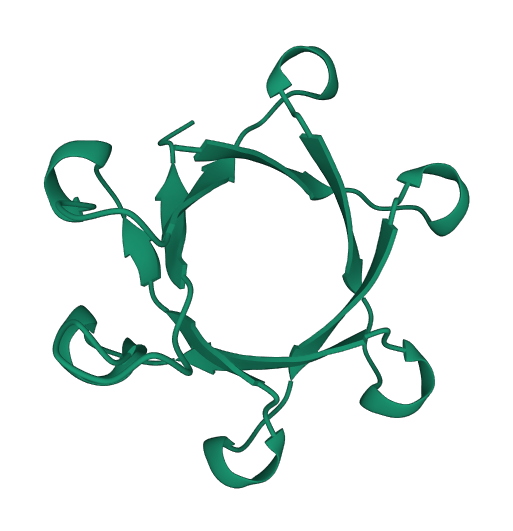
\includegraphics[width=0.5\textwidth]{figures/Figure1_A0A165M1R5F1_PUD1_2_domain-containing_protein.png}
\caption{Example of a knotted protein: A0A165M1R5 protein (\textit{Acidovorax} sp.), featuring a 7$_1$ knot, as predicted by ESMFold \citep{lin2023evolutionary}.}
\label{fig:knotted_protein}
\end{figure}

Knotted proteins are a unique class of proteins in which the backbone forms a knot-like structure, example on Figure~\ref{fig:knotted_protein}. Imagine pulling on both ends of a protein chain like a piece of string—if the protein is knotted, it won't come apart \citep{knot_discovery, mishra2012knot}. Such structures offer several advantages:

\textbf{Enhanced stability}: The formation of knots in proteins can significantly enhance the kinetic stability of proteins during folding and unfolding processes \citep{lua2012pyknot}, \citep{a2013folding}. Knotted proteins are often more resistant to mechanical degradation by proteolytic machines like ClpP/X, which could provide a survival benefit in various cellular contexts \citep{soler2013effects}. 

\textbf{Unique functional properties}: The complex topology creates distinctive active sites and binding pockets, contributing to enzymatic activity and substrate specificity \citep{king2007identification}.  For example, the enzyme N-acetylornithine transcarbamylase (AOTCase), which possesses a knot, showcases how topology can affect enzymatic pathways, leading to different substrate processing compared to its homologues without knot \citep{brems2022alphafold}.

\textbf{Evolutionary conservation}: The preservation of knots across species and within protein families suggests functional importance, indicating these complex topologies provide selective advantages \citep{brems2022alphafold}, \citep{begun2024effect}, \citep{puri2022elucidation}. 

Despite these intriguing properties, the rarity of knotted proteins in nature poses challenges for their study. Recent advances in AI-driven protein design have demonstrated the possibility of generating knotted proteins: \citep{klimentova2024unveiling} combined RFdiffusion \& ProteinMPNN together with EvoDiff, discovering three knot types (5$_1$, 7$_4$, and 8$_{19}$) not previously observed in natural proteins, \citep{watson2023novo}, \citep{dauparas2022robust}, \citep{alamdari2023protein}. However, these approaches suffered from low success rates ($\sim 0.5$\% success rate for generating knotted proteins) and lacked control over the generation process.

The recent release of ESM3 \citep{hayes2025simulating}, a frontier-scale multi-modal protein language model, offers new opportunities for controlled protein design. ESM3 unifies multiple protein modalities—sequence, structure, and function—in a single framework, enabling capabilities that previously required multiple specialized tools: structure prediction (AlphaFold2), inverse folding (ProteinMPNN), and structure generation (RFdiffusion). Its ability to perform guided generation based on scoring functions makes it particularly suitable for targeting rare protein features like knots.

In this work, we leverage ESM3 to address the challenge of knotted protein design through three key contributions: (1) We introduce a continuous knot score metric that quantifies the robustness of protein knots, moving beyond binary classification; (2) We demonstrate ESM3-guided generation achieving 87\% success rate in producing knotted proteins, a dramatic improvement over previous methods; (3) We show that ESM3 embeddings enable highly accurate classification and facilitate the transformation of unknotted proteins into knotted variants through iterative modifications.

\section{Methods}

We took advantage of previously published data on 1,000 knotted and 4,000 unknotted real proteins from \texttt{EvaKlimentova/Diffusion-all\_knots} dataset stored at HuggingFace Hub\footnote{\url{https://huggingface.co/datasets/EvaKlimentova/Diffusion-all_knots}}. The code used for the analysis was uploaded to GitHub repository \url{https://github.com/ML-Bioinfo-CEITEC/KPDwESM3}. Experiments were conducted on a virtual machine equipped with an NVIDIA A100 GPU, 16 CPU cores, and 64 GB of memory.

\subsection{ESM3 Model and Guided Generation}

We employed the open-source ESM3-SM (1.4B parameters) model. While larger models may exhibit higher fidelity in structure generation, the ESM3-SM provides an effective platform for demonstrating the key capabilities of the multi-modal architecture:
\begin{itemize}
    \item \textbf{Structure prediction}: sequence $\rightarrow$ structure
    \item \textbf{Inverse folding}: structure $\rightarrow$ sequence
    \item \textbf{Masked sequence prediction}: partially masked sequence $\rightarrow$ sequence
    \item \textbf{Embeddings}: sequence $\rightarrow$ learned representations
    \item \textbf{Guided generation}: conditional sampling with custom scoring functions
\end{itemize}

The methods presented here are model-agnostic and are expected to show continued success when applied to larger-scale models as they become publicly available (like EMS3 7B and 98B models).

For guided generation of knotted proteins, we implement a scoring function $s(x)$ that evaluates the knottedness of generated structures using the Topoly Python package with Alexander polynomials \url{https://github.com/ilbsm/topoly_tutorial}. The generation process follows:
\begin{equation}
p(x|c) \propto p(x) \cdot \exp(\lambda \cdot s(x))
\end{equation}
where $p(x)$ is the base ESM3 distribution, $c$ represents conditioning information, $s(x)$ is the knot metric (either original or smoothed) and $\lambda$ controls the strength of guidance. 

\subsection{Continuous Knot Score}

Traditional knot detection provides binary labels (knotted/unknotted). To quantify knottiness, we first process Topoly output by extracting probabilities for all predicted topologies and calculating the proportion of trivial topology (0\_1, unknotted).

We then propose a continuous knot score that captures the robustness of protein knots through randomized masking - see Algorithm 1.

\begin{algorithm}[tb]
   \caption{Randomized Knot Score Calculation}
   \label{alg:knot_score}
\begin{algorithmic}
   \STATE {\bfseries Input:} protein sequence $s$, masking perc. $X$, trials $N$
   \STATE {\bfseries Output:} knot\_score $\in [0, 1]$
   \STATE Initialize $knotted\_sum = 0$
   \FOR{$i=1$ {\bfseries to} $N$}
   \STATE Randomly mask $X\%$ of sequence $s$ $\rightarrow$ $s_{masked}$
   \STATE Generate masked regions using ESM3 $\rightarrow$ $s_{generated}$
   \STATE Predict structure of $s_{generated}$ using ESM3
   \STATE Calculate topology using Topoly
   \STATE $knotted\_sum = knotted\_sum + P(topology \neq 0\_1)$
   \ENDFOR
   \STATE {\bfseries Return} $knot\_score = knotted\_sum / N$
\end{algorithmic}
\end{algorithm}

For our analysis, we use $X=10\%$ masking and $N=16$ trials. The knot score is then defined as:
\begin{equation}
\text{knot\_score} = \frac{1}{N} \sum_{i=1}^{N} \mathbb{P}[\text{topology}_i \neq 0\_1]
\end{equation}
where $\mathbb{P}[\text{topology}_i \neq 0\_1]$ is the probability of knottiness. This score ranges from 0 (robustly unknotted) to 1 (robustly knotted), providing nuanced information about borderline cases.

\subsection{Knot Stability Analysis}

To assess knot stability, we systematically analyze how much sequence modification is required to break a knot. For each of 1,000 knotted proteins, we apply masking percentages from 5\% to 95\% in 5\% increments. For each masking percentage, we perform 16 independent trials and calculate the randomized knot score. We define the "breaking point" as the masking percentage where the knot score falls below 0.75.

\subsection{Guided Protein Generation and Transformation}

We implement two distinct protocols for working with knotted proteins:

\textbf{(a) De novo generation of knotted proteins:}
Starting from a fully masked sequence, we use guided generation with $\lambda=1.0$ and the knot score as the objective function to directly generate knotted proteins.

\textbf{(b) Unknotted-to-knotted transformation:}
We start with an unknotted protein sequence and iteratively modify it through guided generation. In each iteration, we randomly mask 5\% of the sequence and apply guided regeneration to these masked regions using the knot score as the objective. This process continues for up to 10 iterations or until the protein achieves a knot score above 0.8, indicating a successful transformation to a knotted structure.

\subsection{Knot Classification Using ESM3 Embeddings}

To evaluate the discriminative power of ESM3 representations for knot detection, we train a neural network classifier. We use 1,000 knotted proteins from our dataset with sequences masked and regenerated from 5\% to 95\%, creating a dataset of 383,523 training proteins and 42,613 validation proteins. Different proteins were used for training and validation masking to prevent data leakage. Both datasets contain approximately 73\% knotted proteins.

We extract ESM3 embeddings (dimension 1,536) using sequences only and train a fully connected neural network with two hidden layers (1,024 and 256 neurons) for binary classification (knotted vs. unknotted).



\section{Results}

\subsection{ESM3 Embeddings Enable Accurate Knot Classification}

We first evaluated whether ESM3's learned representations capture topological information. Training a simple neural network classifier on ESM3 sequence embeddings, we achieved 93\% accuracy in distinguishing knotted from unknotted proteins, see Table \ref{confusion-matrix}. This high accuracy suggests that ESM3 implicitly learns topological features despite not being explicitly trained on knot labels.

\begin{table}[h]
\caption{Confusion matrix on the validation set. The model achieves 93\% accuracy in identifying knotted proteins.}
\label{confusion-matrix}
\vskip 0.15in
\begin{center}
\begin{small}
\begin{sc}
\begin{tabular}{lcc}
\toprule
True vs. Predicted &  Unknotted & Knotted \\
\midrule
 Unknotted & 10644 & 866 \\
 Knotted & 1924  & 29179 \\
\bottomrule
\end{tabular}
\end{sc}
\end{small}
\end{center}
\vskip -0.1in
\end{table}

\subsection{Knot Topology is Robust to Sequence Perturbation}

Our analysis showed that knots are remarkably stable under sequence perturbation. On average, more than 80\% of a protein's sequence must be altered to disrupt the knot (Figure \ref{fig:stability}), indicating that the core topological information is preserved within a fraction of the original sequence.

\begin{figure}[h]
\centering
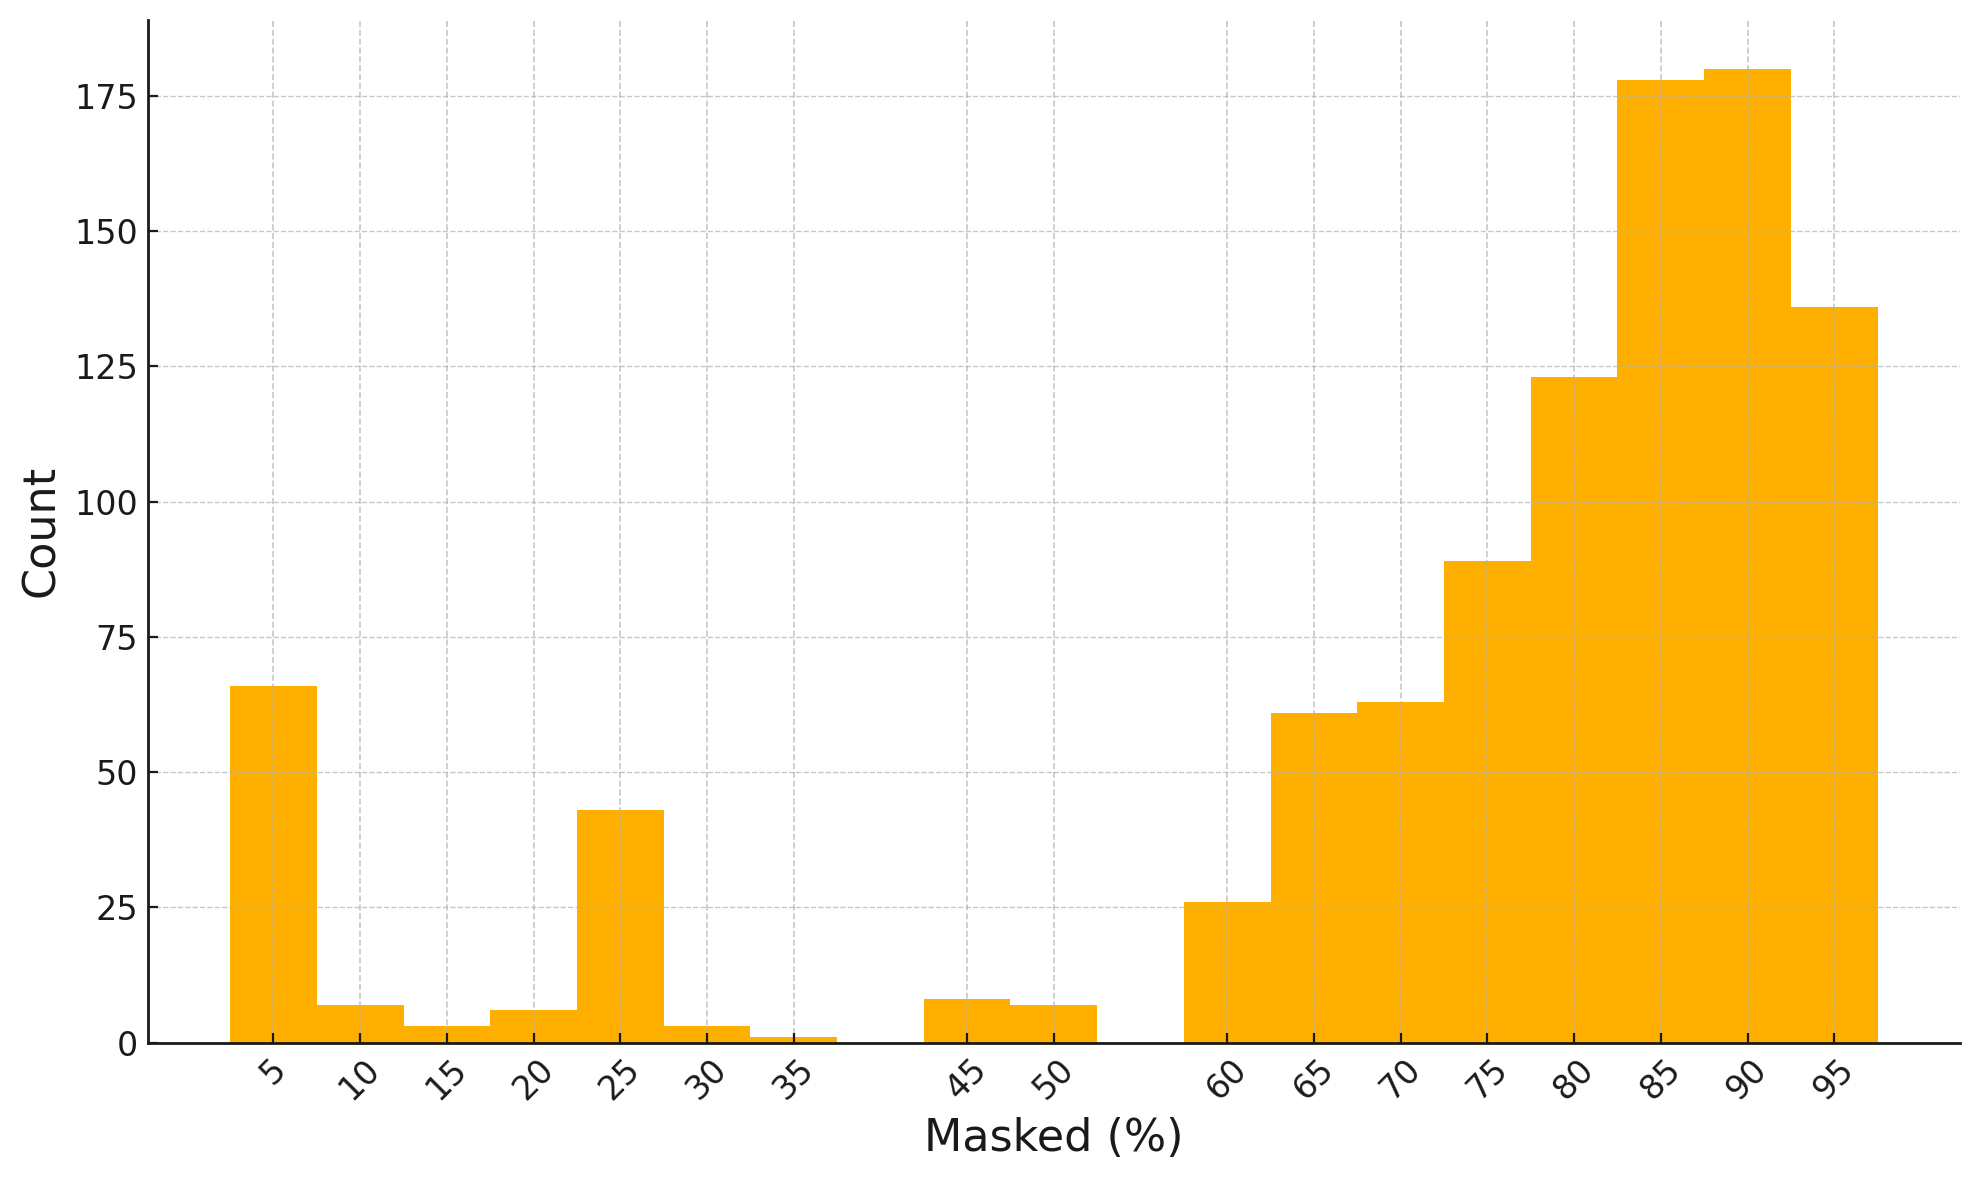
\includegraphics[width=0.5\textwidth]{figures/Fig2hist.png}
\caption{Histogram of percentage of sequence that must be masked to break the knot.}
\label{fig:stability}
\end{figure}


What we originally expected was a smooth decrease in the knot score from one to zero, as in Figure \ref{fig:stability2}. 

\begin{figure}[h]
\centering
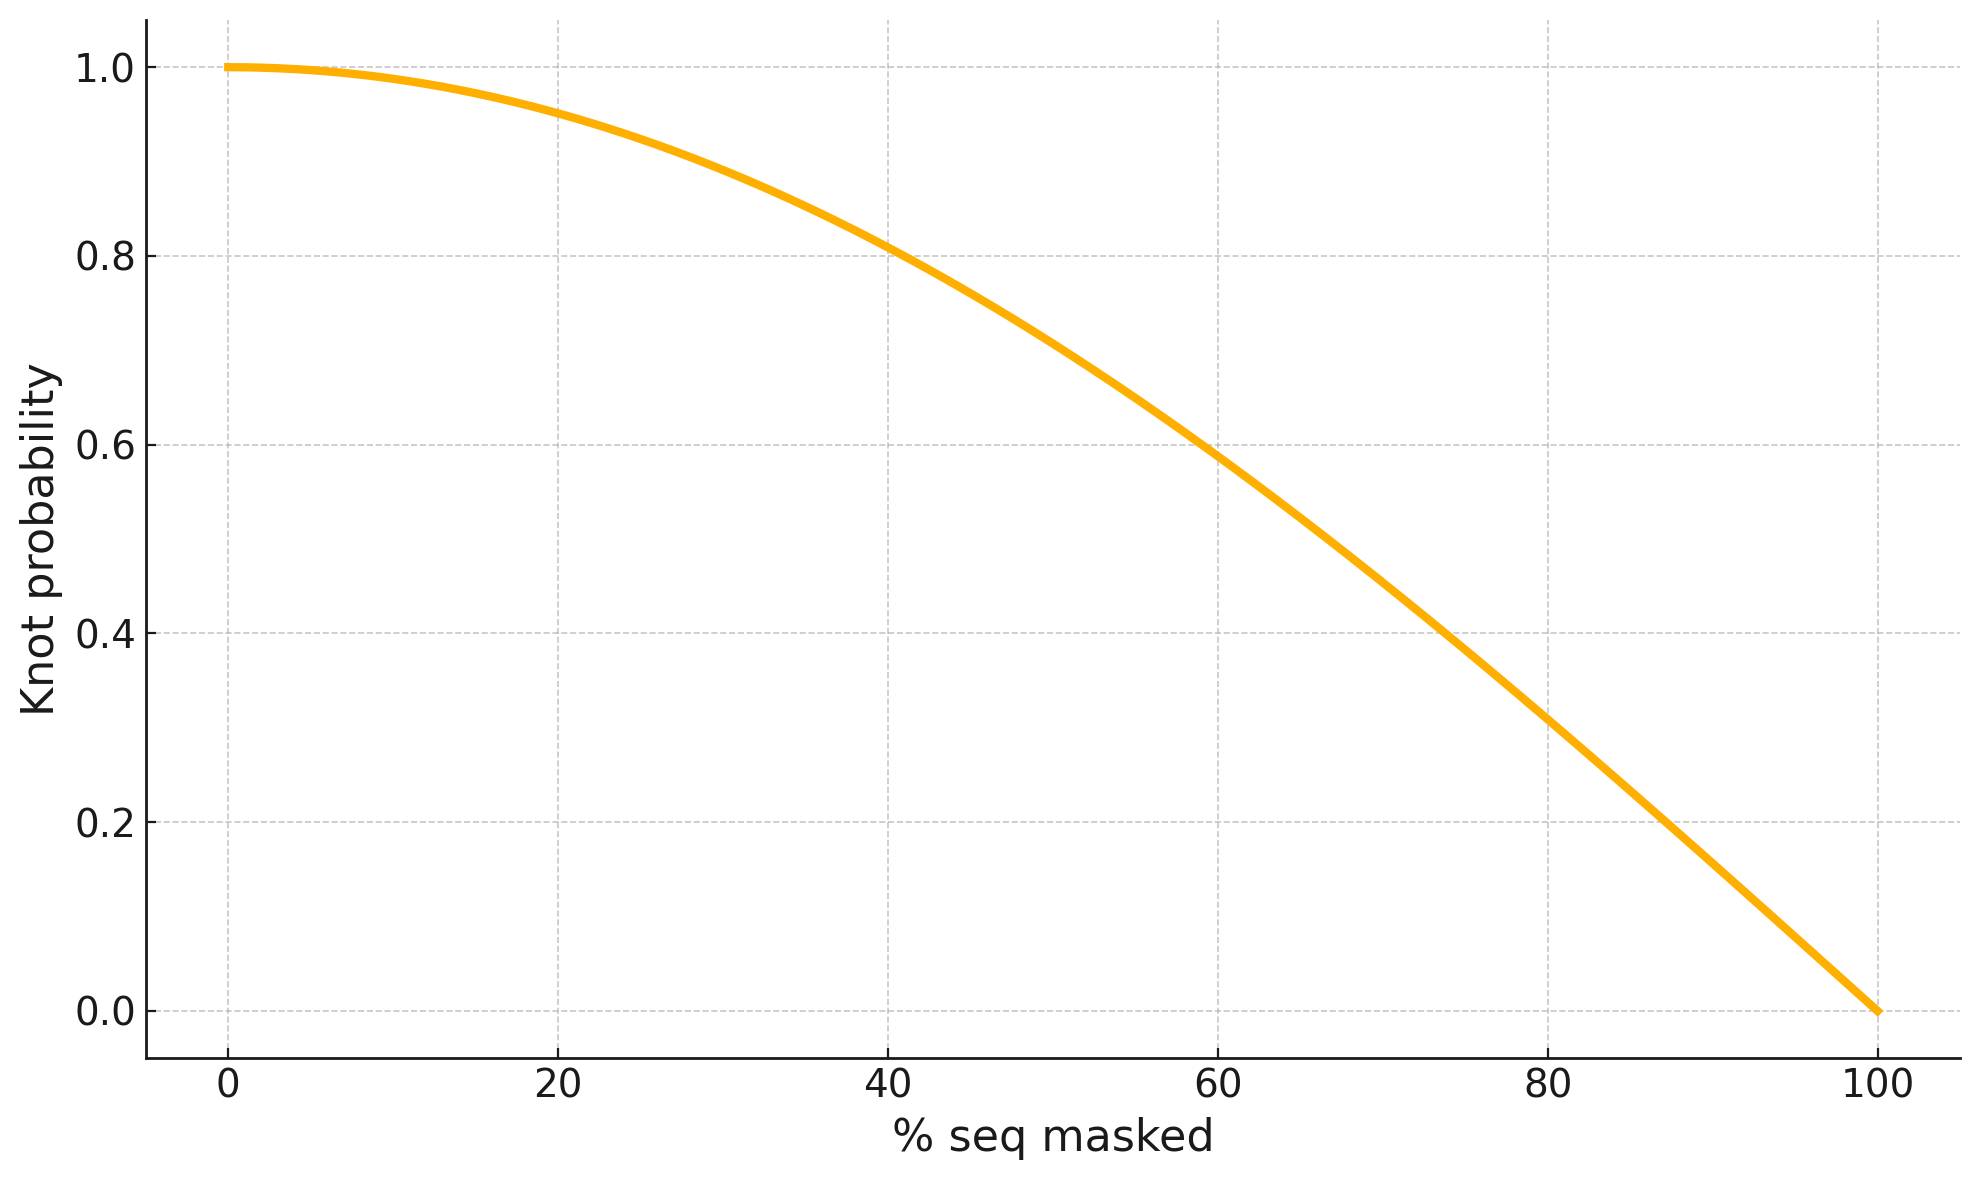
\includegraphics[width=0.45\textwidth]{figures/Fig3expected.png}
\caption{Expected dependence of knot probability on percentage of masking may look like.}
\label{fig:stability2}
\end{figure}

In fact, the probability of maintaining the knot drops sharply around the breaking point, indicating that a critical threshold is needed for topological stability, see Figure \ref{fig:stability3}.

\begin{figure}[h]
\centering
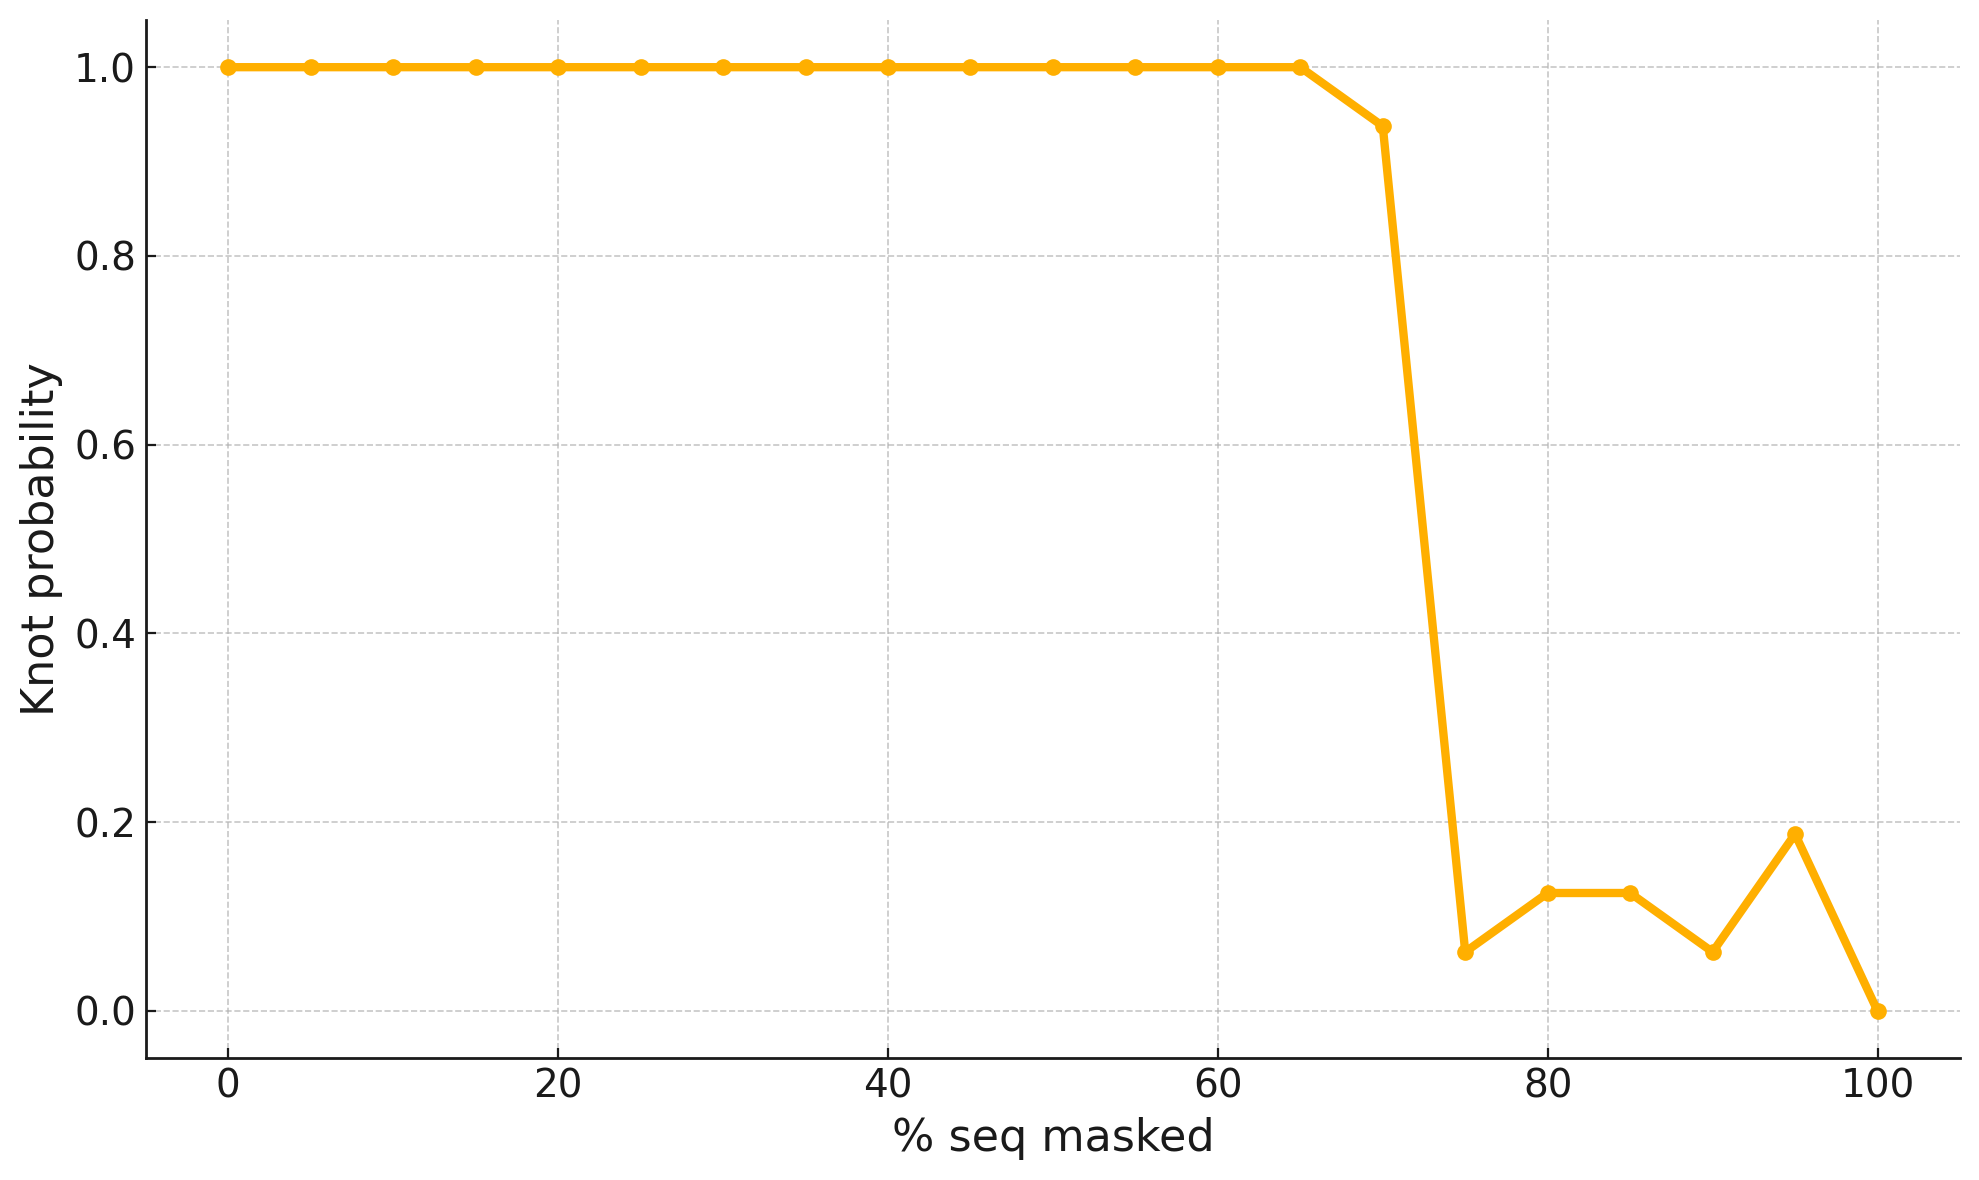
\includegraphics[width=0.45\textwidth]{figures/Fig4actual.png}
\caption{Observed dependence of knot probability on masking percentage for a representative protein.}
\label{fig:stability3}
\end{figure}


\subsection{Guided Generation Achieves 87\% Success Rate}

Using ESM3's guided generation capabilities, we achieved an 87\% success rate in generating knotted proteins; see the example in Figure \ref{fig:generated}. 

\begin{figure}[h!]
\centering
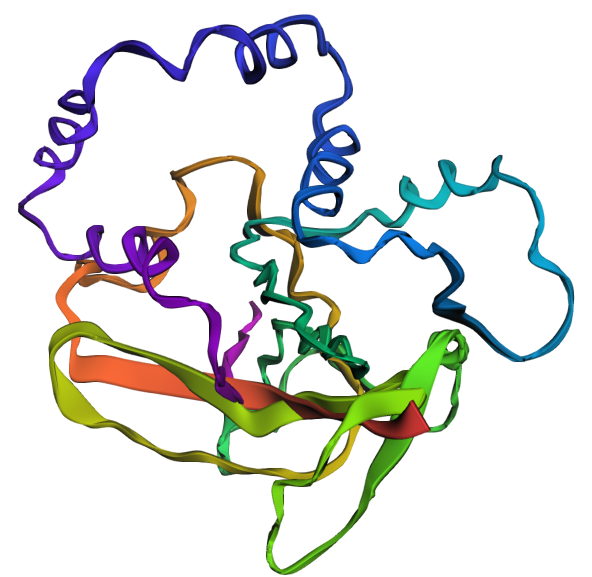
\includegraphics[width=0.4\textwidth]{figures/Figure5v3.png}
\caption{Example of generated knotted protein.}
\label{fig:generated}
\end{figure}

This represents $\sim 170$-fold improvement over the unguided approaches ($\sim 0.5\%$ success rate) used in previous work.

Our iterative modification protocol successfully converted 31\% of unknotted proteins into knotted variants. Successful transformations typically required 3-5 iterations.

\section{Discussion and Conclusion}

This work demonstrates the transformative potential of multi-modal foundation models like ESM3 for complex protein design tasks. By unifying sequence, structure, and function modeling in a single framework, ESM3 enables capabilities that previously required multiple specialized tools, while adding powerful new features like guided generation.

The finding that a large majority of sequence must be modified to break the knot has implications for understanding knot evolution and designing stable knotted proteins for applications. We verified that ESM3 is not simply memorizing sequences and the generated knotted proteins differ significantly from their original counterparts.

The dramatic improvement in generation success rate (from 0.5\% to 87\%) showcases the power of guided generation for targeting rare protein features. This success was achieved despite several simplifications in our approach. First, our random masking strategy did not distinguish between the knot core and terminal regions. Second, we did not incorporate secondary structure information or spatial proximity relationships in our generation process. A more sophisticated masking strategy that accounts for topological importance could potentially improve both generation success rates and the functional relevance of designed proteins.

While we acknowledge the limitations of using the smaller open-source ESM3 model, the techniques presented here are model-agnostic. Their relevance is underscored by the emergence of powerful new foundation models, such as Boltz \citep{wohlwend2024boltz} and AlphaFold3 \citep{abramson2024accurate}, which are increasingly capable of integrating diverse biological data. The high accuracy (93\%) we achieved in knot classification using only sequence embeddings suggests that these larger models will likely capture even more subtle topological features with greater fidelity.

\section*{Impact Statement}

Our results highlight how multi-modal foundation models are reshaping protein design, enabling precise control over complex structural features that were previously accessible only through undirected sampling. As these models continue to scale and improve, we anticipate even greater capabilities for engineering proteins with desired topological and functional properties. The ability to generate genuinely novel knotted proteins—rather than minor variants of known sequences—opens new avenues for creating proteins with enhanced stability and unique functional properties for biotechnological applications.

\section*{Acknowledgments}
The project was supported by the OPUS LAP program of the Czech Science Foundation, project no. 23-04260L (“Biological code of knots – identification of knotted patterns in biomolecules via AI approach”). Computational resources were supplied by the project "e-Infrastruktura CZ" (e-INFRA CZ LM2018140) supported by the Ministry of Education, Youth and Sports of the Czech Republic.

\bibliography{references}
\bibliographystyle{icml2025}

\end{document}